\secrel{Smart Watch}\ \\

\noindent
\begin{tabular}{l p{0.75\textwidth}}
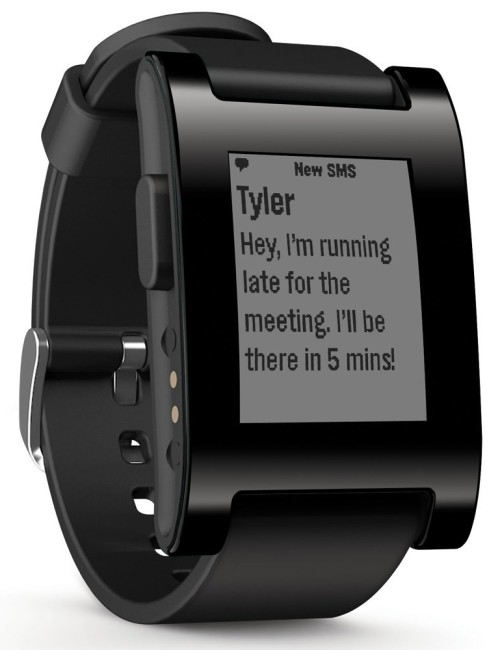
\includegraphics[height=0.45\textheight,valign=t]{img/pebble_classic.png}
&
I have this one Pebble Classic myself. It's an old smartwatch, which has BT
connection with host software on the mobile phone but can work standalone a long
time (more than two weeks without recharge). It is lightweight, adjustable and
can be good terminal for instant planning.
\\
\end{tabular}
This device was done on a light SMT32 microcontroller, and you can program it in
pure C using online Pebble SDK. It was not treated as one of targets for \uF, as
it has no keyboard or remote terminal. Here I
\href{https://www.quora.com/unanswered/How-can-I-write-remote-terminal-Android-for-Pebble-Classic-Smartwatch-to-be-able-to-reprogram-it-interactively-I-think-about-full-watch-hosted-Forth-port-or-tiny-bytecode-interpreter-and-compiler-embedded-into-the}{asked
about terminal} able to work on mobile phone, and let to interact with Pebble in
a live session. Still have no working decision.
